\section{ZnO Substrate Yields the Best Ag Thin Film}

In this section, we will answer the question that  which substrate type is best for Ag thin film deposition. Three different bond length will be used: 3.3$\angstrom$, 2.9$\angstrom$, 2.3$\angstrom$. 3.3$\angstrom$ is equivalent to ZnO lattice constant. 2.9$\angstrom$ is for Ag bond length, which means this substrate has a zero misfit for Ag thin film. At last, 2.3$\angstrom$ is selected for simulating a negative lattice mismatch factor, where lattice mismatch factor($f_{mismatch}$) is defined via:
\begin{align}
    f_{mismatch} = \frac{a_{substrate} - a_{film}}{a_{substrate}}
    \label{Chap:Ag/ZnO:eq:mismatch}
\end{align}

\begingroup
\begin{figure}[!ht]
  \centering
  \subfigure[]{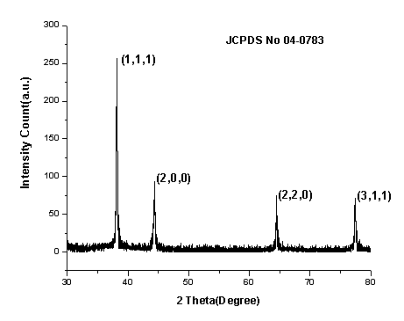
\includegraphics[width=0.45\linewidth]{Chap4/plots/Picture4a.pdf}}\label{Chap:Ag/ZnO:fig:4a}
  \subfigure[]{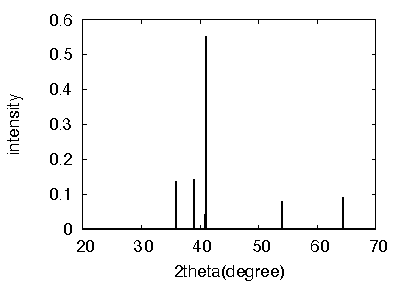
\includegraphics[width=0.45\linewidth]{Chap4/plots/Picture4b.pdf}}\label{Chap:Ag/ZnO:fig:4b}
\caption[XRD plots of FCC and HCP Ag]{XRD plots of FCC and HCP Ag. (a) XRD results of Ag with labeled peaks from JCPDS. \cite{AgPDF} (b) Simulated XRD results for HCP Ag.}
  \label{Chap:Ag/ZnO:fig4}
\end{figure}
\endgroup

In order to characterize the orientation of thin films, simulated \ac{XRD} will be evaluated. As shown in Fig. \ref{Chap:Ag/ZnO:fig:4a}, Ag {111} orientation will have a strong peak around $38^{\circ}$. We also simulated \ac{XRD} results for \ac{HCP} Ag in order to characterize the crystalline quality of Ag thin films. And we can see if Ag is in \ac{HCP} structure, there will be strong peaks around $35.86^{\circ}$, $38.95^{\circ}$, and $40.96^{\circ}$.

\begingroup
\begin{figure}[!ht]
  \centering
  \subfigure[]{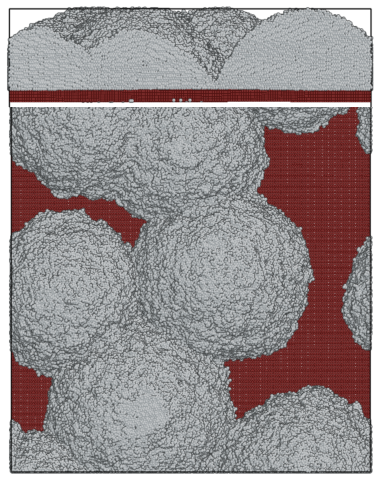
\includegraphics[width=0.32\linewidth]{Chap4/plots/Picture5a.pdf}}\label{Chap:Ag/ZnO:fig:5a}
  \subfigure[]{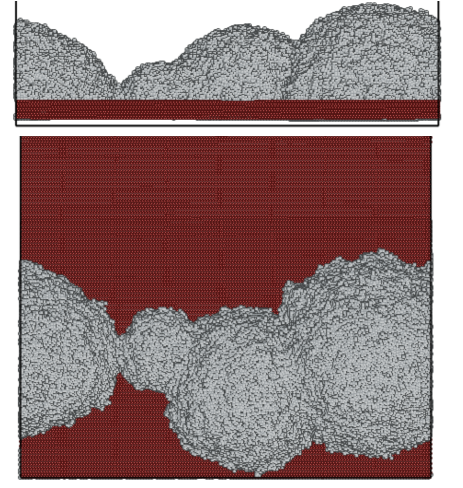
\includegraphics[width=0.32\linewidth]{Chap4/plots/Picture5b.pdf}}\label{Chap:Ag/ZnO:fig:5b}
  \subfigure[]{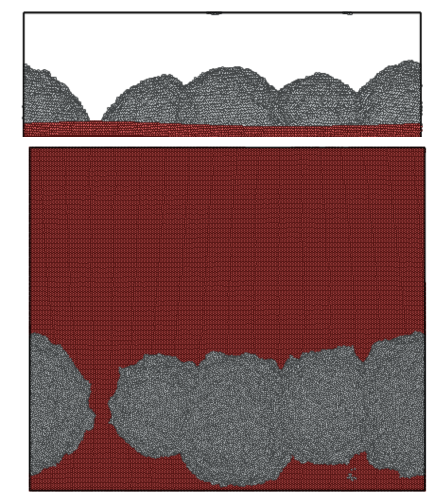
\includegraphics[width=0.32\linewidth]{Chap4/plots/Picture5c.pdf}}\label{Chap:Ag/ZnO:fig:5c}
\caption[GCMC simulated Ag thin film morphology on hexagonoal substrates.]{GCMC simulated Ag thin film morphology on hexagonoal substrates with bond length of (a) 2.3$\angstrom$, (b) 2.9$\angstrom$, and (c) 3.3$\angstrom$. Top sub-figures are side views of 30 ML atoms and bottom sub-figures are top views.}
  \label{Chap:Ag/ZnO:fig5}
\end{figure}
\endgroup

We first investigate the results of hexagonal substrate with 3 different bond length, as shown in Fig. \ref{Chap:Ag/ZnO:fig5}. 